\maketitle
\section{Descripción del método.}
El método recibe un conjunto de puntos, dados de una función desconocida y realiza interpolación polinomial. El método utiliza el polinomio de Vandermonde, de Newton y de Lagrange \cite{interp}. Posteriormente, como se quiere aproximar la raíz de la función desconocida, se realiza el siguiente procedimiento a los \textbf{tres} polinomios interpolantes: se hace una búsqueda de un segmento de recta que tenga un cambio de signo al evaluar los extremos en los polinomios; a partir de este segmento de recta se realiza bisección hasta encontrar la raíz. Este segmento de recta se encuentra utilizando el algoritmo Nelder-Mead \cite{Singer2009}, que, como se está trabajando en una dimensión, lo busca a partir de líneas, que se reflejan, expanden o contraen basado en los valores de losw vértices.

\section{Ejemplo y Resultados.}
Para el ejemplo se utilizó la siguiente función en el intervalo $[-1,4]$, cuya gráfica se muestra en la figura \ref{fig:example}.
\begin{equation}
    y(t) = e^{-t/2}\cos(2t)
\end{equation}
\begin{figure}[H]
    \centering
    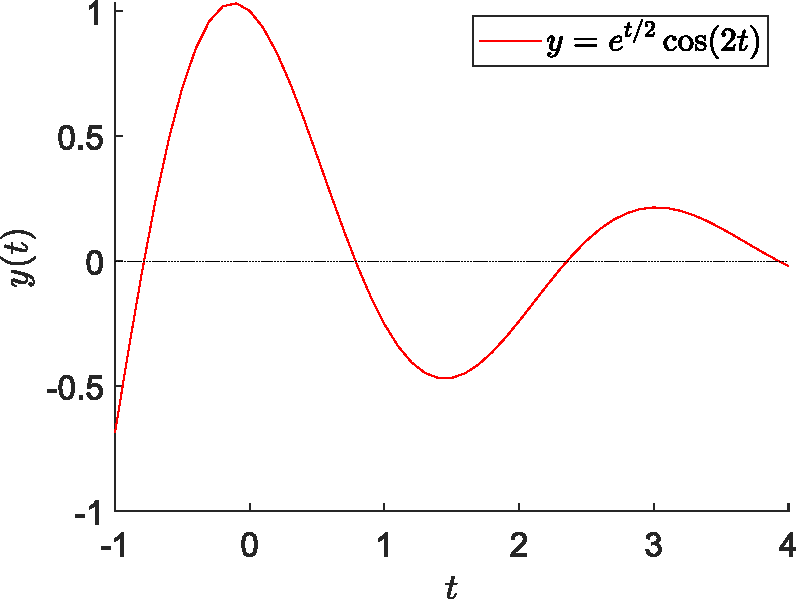
\includegraphics[scale=0.6]{funct.pdf}
    \caption{Función ejemplo.}
    \label{fig:example}
\end{figure}
De este gráfico, se puede observar que la función tiene cuatro raíces en el intervalo $[-1,4]$.

\subsection{Aproximación por 6 Puntos}
Se seleccionó el siguiente conjunto de 6 puntos:
\begin{table}[H]
\centering
\begin{tabular}{cc}
\hline
$\boldmath{t}$ & $\boldmath{y(t)}$ \\ \hline
-1.0           & -0.6861           \\
0.0            & 1.0000            \\
1.0            & -0.2524           \\
2.0            & -0.2405           \\
3.0            & 0.2142            \\
4.0            & -0.0197           \\ \hline
\end{tabular}
\caption{Puntos seleccionados.}
\label{tab:6points}
\end{table}
Y el polinomio interpolante obtenido por los tres métodos es:
\begin{equation}
    P(t)=0.0393 t^5 - 0.4058 t^4 + 1.3156 t^3 - 1.0635 t^2 - 1.1381 t + 1.000
\end{equation}
Que genera una aproximación regular de la función en el intervalo $[-1,4]$, como se muestra en la figura \ref{fig:graph6points}.
\begin{figure}[H]
    \centering
    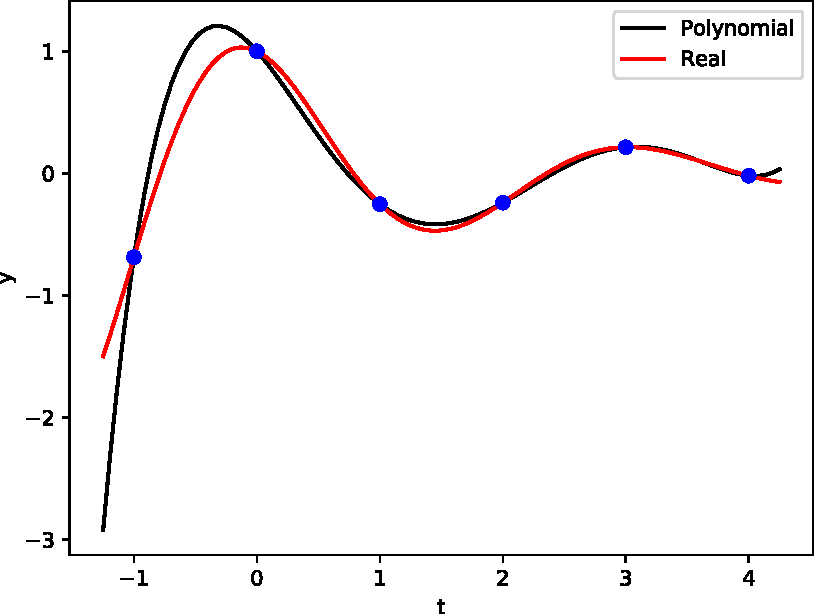
\includegraphics[scale=0.6]{6_points_polynomial.pdf}
    \caption{Función original vs. polinomio interpolante.}
    \label{fig:graph6points}
\end{figure}


\subsection{Aproximación por 9 Puntos}
Se seleccionó el siguiente conjunto de 9 puntos:
\begin{table}[H]
\centering
\begin{tabular}{cc}
\hline
$\boldmath{t}$ & $\boldmath{y(t)}$ \\ \hline
-1.000           & -0.6861           \\
-0.375         & 0.8826            \\
0.250           & 0.7745            \\
0.875          & -0.1151           \\
1.500           & -0.4676           \\
2.125          & -0.1542           \\
2.750           & 0.1792            \\
3.375          & 0.1652            \\
4.000            & -0.0197           \\ \hline
\end{tabular}
\caption{Puntos seleccionados.}
\label{tab:9points}
\end{table}
Matriz de Vandermonde:
\begin{equation*}
    \left[
    \begin{smallmatrix}
1 & -1 &  1  &  -1 &  1 &  -1 &  1 &  -1 &  1\\
3.9107\times10^{-4} & -1.0428\times10^{-3} &  2.7809\times10^{-3} &  -7.4158\times10^{-3} &  1.9775\times10^{-2} &  -5.2734\times10^{-2} &  1.4062\times10^{-1} &  -3.7500\times10^{-1} &  1\\
1.5259\times10^{-5} &  6.1035\times10^{-5} &  2.4414\times10^{-4} &  9.7656\times10^{-4} &  3.9062\times10^{-3} &  1.5625\times10^{-2} &  6.2500\times10^{-2} &  2.5000\times10^{-1} &  1\\
3.4361\times10^{-1} &  3.9270\times10^{-1} &  4.4880\times10^{-1} &  5.1291\times10^{-1} &  5.8618\times10^{-1} &  6.6992\times10^{-1} &  7.6562\times10^{-1} &  8.7500\times10^{-1} &  1\\
2.5629\times10^{+1} &  1.7086\times10^{+1} &  1.1391\times10^{+1} &  7.5938 &  5.0625 &  3.3750 &  2.2500 &  1.5000 &  1\\
4.1579\times10^{+2} &  1.9566\times10^{+2} &  9.2078\times10^{+1} &  4.3331\times10^{+1} &  2.0391\times10^{+1} &  9.5957 &  4.5156 &  2.1250 &  1\\
3.2709\times10^{+3} &  1.1894\times10^{+3} &  4.3251\times10^{+2} &  1.5728\times10^{+2} &  5.7191\times10^{+1} &  2.0797\times10^{+1} &  7.5625 &  2.7500 &  1\\
1.6834\times10^{+4} &  4.9879\times10^{+3} &  1.4779\times10^{+3} &  4.3789\times10^{+2} &  1.2975\times10^{+2} &  3.8443\times10^{+1} &  1.1391\times10^{+1} &  3.3750 &  1\\
6.5536\times10^{+4} &  1.6384\times10^{+4} &  4.0960\times10^{+3} &  1.0240\times10^{+3} &  2.5600\times10^{+2} &  6.4000\times10^{+1} &  1.6000\times10^{+1} &  4.0000 &  1
    \end{smallmatrix}
    \right]
\end{equation*}


Matriz de Newton:

\begin{equation*}\left[
    \begin{smallmatrix}
8.9081\times10^{-1} & 0.0000 & 0.0000 & 0.0000 & 0.0000 & 0.0000 & 0.0000 & 0.0000 & 0.0000\\
1.1224 & 3.7056\times10^{-1} & 0.0000 & 0.0000 & 0.0000 & 0.0000 & 0.0000 & 0.0000 & 0.0000\\
8.5506\times10^{-1} & -4.2775\times10^{-1} & -6.3865\times10^{-1} &  0.0000 &  0.0000 & 0.0000 & 0.0000 & 0.0000 & 0.0000\\
4.1386\times10^{-1} & -7.0593\times10^{-1} & -2.2254\times10^{-1} &  2.2192\times10^{-1} &  0.0000 & 0.0000 & 0.0000 & 0.0000 & 0.0000\\
3.3414\times10^{-2} & -6.0871\times10^{-1} & 7.7771\times10^{-2} &  1.6017\times10^{-1} & -2.4703\times10^{-2} & 0.0000 &  0.0000 & 0.0000 & 0.0000\\
-1.8187\times10^{-1} & -3.4446\times10^{-1} &  2.1140\times10^{-1} &  7.1270\times10^{-2} & -3.5558\times10^{-2} & -3.4737\times10^{-3} &  0.0000 &  0.0000 & 0.0000\\
-2.3370\times10^{-1} & -8.2924\times10^{-2} &  2.0923\times10^{-1} & -1.1598\times10^{-3} & -2.8972\times10^{-2} &  2.1077\times10^{-3} &  1.4884\times10^{-3} & 0.0000 & 0.0000\\
-1.7997\times10^{-1} & 8.5976\times10^{-2} &  1.3512\times10^{-1} & -3.9524\times10^{-2} & -1.5346\times10^{-2} &  4.3604\times10^{-3} &  6.0071\times10^{-4} & -2.0289\times10^{-4} & 0.0000\\
-8.8461\times10^{-2} & 1.4641\times10^{-1} &  4.8345\times10^{-2} & -4.6280\times10^{-2} & -2.7022\times10^{-3} &  4.0460\times10^{-3} & -8.3839\times10^{-5} & -1.5647\times10^{-4} &  9.2843\times10^{-6}
    \end{smallmatrix}\right]
\end{equation*}

Y el polinomio interpolante obtenido por los tres métodos es:
\begin{equation*}
    P(t)=(-4.5636\times 10^{-5}) t ^8 - 0.0069  t ^7 + 0.0910  t ^6 - 0.3770  t ^5 + 0.3515  t ^4 + 1.1224  t ^3 - 1.9172  t ^2 - 0.5210  t + 1.0060
\end{equation*}
Que genera una muy buena aproximación de la función en el intervalo $[-1,4]$, como se muestra en la figura \ref{fig:graph9points}.
\begin{figure}[H]
    \centering
    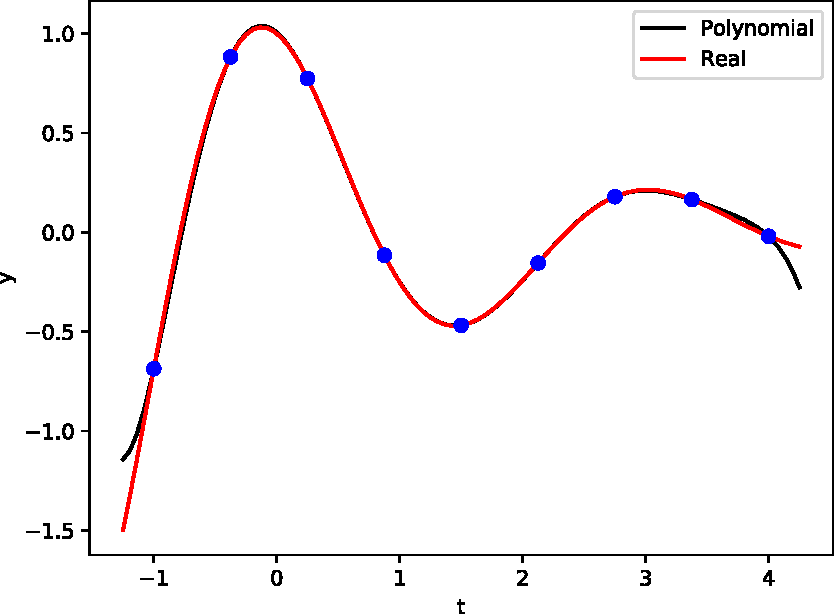
\includegraphics[scale=0.6]{9_points_polynomial.pdf}
    \caption{Función original vs. polinomio interpolante.}
    \label{fig:graph9points}
\end{figure}


Para aproximar la raíz, se utilizó el proceso ya descrito y se obtuvo un resultado exitoso, hallando la raíz de la función correspondiente a $\pi/4$, como se muestra en la figura \ref{fig:root1}.
\begin{figure}[H]
    \centering
    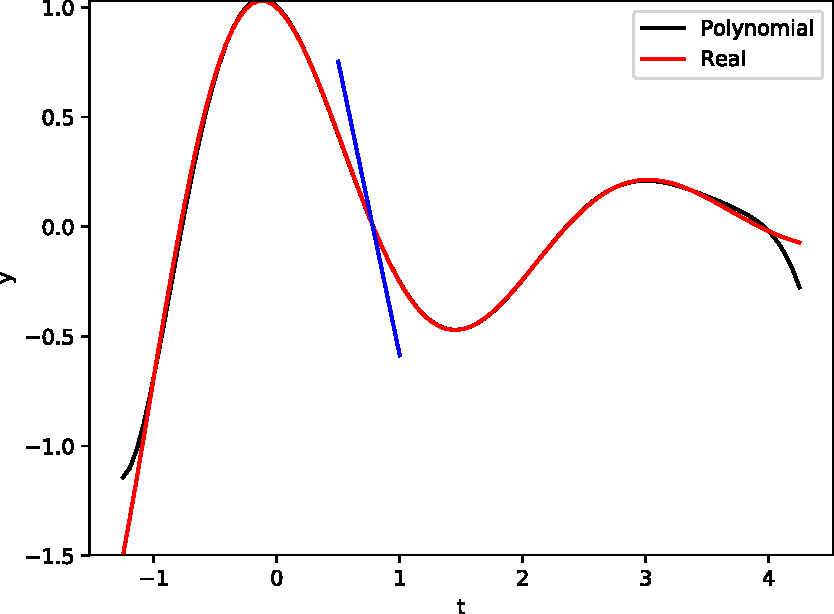
\includegraphics[scale=0.5]{Solution_1.pdf}
    \caption{Raíz encontrada.}
    \label{fig:root1}
\end{figure}

\subsection{Ejemplo 15 puntos}
Este ejemplo es para mostrar más claramente el método para encontrar las raíces. Para este ejemplo se utilizó la función en el intervalo $[-3,3]$.
\begin{equation}
    f(t)=x\cos(x)+e^{-2t}\sin(3t)
\end{equation}
El método se utilizó con una línea inicial determinada y como la línea ya contenía una raíz, se encontró fácilmente. Esto se muestra en la siguiente figura:
\begin{figure}[H]
    \centering
    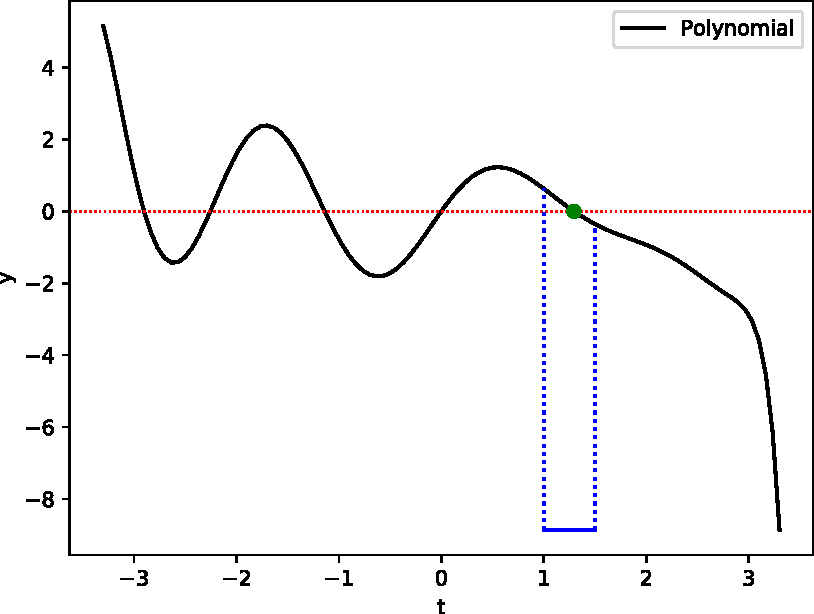
\includegraphics[scale=0.5]{Root_test.pdf}
    \caption{Ejemplo convergencia inmediata.}
\end{figure}

Se utilizó otra línea inicial y como la línea no tenía la raíz, el algoritmo Nelder-Mead iteró hasta encontrar una línea con la raíz. Estos resultados se muestran en la siguiente figura:
\begin{figure}[H]
    \centering
    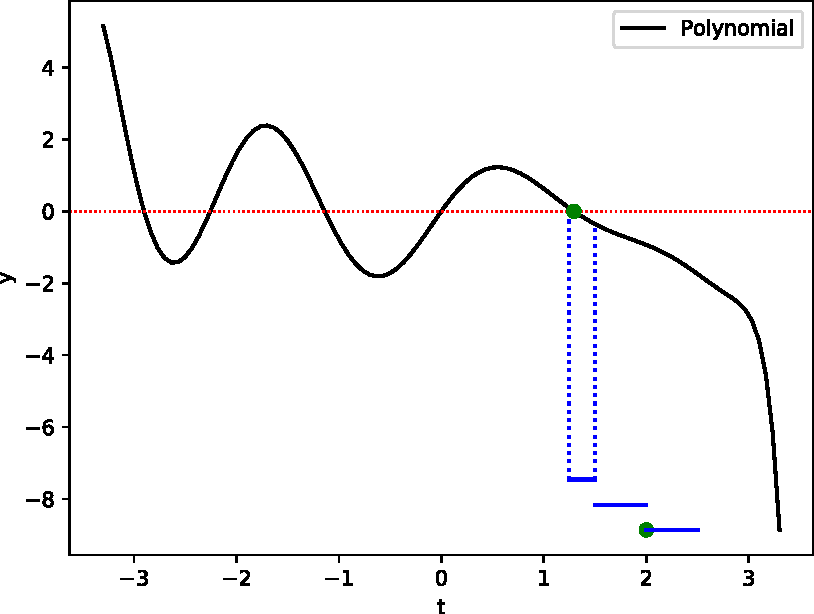
\includegraphics[scale=0.5]{Moving_lines.pdf}
    \caption{Resultados con iteraciones de Nelder-Mead.}
\end{figure}